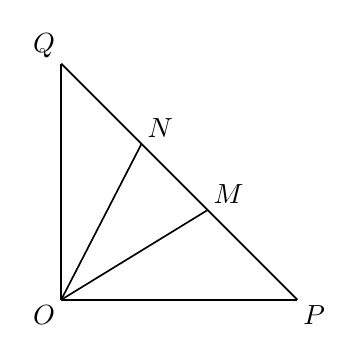
\begin{tikzpicture}[x=1cm,y=1cm,font=\normalsize,
 geometry edge/.style={solid,line width=.6pt},
 geometry mark/.style={solid,line width=.6pt},
 geometry label/.style={font=\normalsize,inner sep=2pt}]
\coordinate (O) at (0,0);
\coordinate (P) at (3,0);
\coordinate (Q) at (0,3);
\coordinate (N) at (1.02,1.98);
\coordinate (M) at (1.86,1.14);
\draw[geometry edge] (O)--(P);
\draw[geometry edge] (O)--(Q);
\draw[geometry edge] (Q)--(N)--(M)--(P);
\draw[geometry edge] (O)--(M);
\draw[geometry edge] (O)--(N);
\node[geometry label,below left] at (O) {$O$};
\node[geometry label,below right] at (P) {$P$};
\node[geometry label,above left] at (Q) {$Q$};
\node[geometry label,above right] at (N) {$N$};
\node[geometry label,above right] at (M) {$M$};
\end{tikzpicture}